% Provenance (never printed): see sources/outline_sources.md (Year 3: elastic waves
% recalled from the physics books; rays in a spherical Earth; travel-time tables;
% surface waves and dispersion; normal modes, told; linear inverse problems and
% seismic tomography). Brief: sources/book5/BRIEFS.md, ch. 1. Curves from
% figdata/bachelor-3/ray_tracing.py, love_dispersion.py, tomo_checkerboard.py;
% exercise and problem values in the Book 5 scratch calculator calc/ch01.py.
\chapter{Sismología e imágenes de la Tierra}\label{ch:b3:seismology-imaging}

El 22 de mayo de 1960, a las 19:11 hora universal, el mayor terremoto registrado desde
1900 rompió la zona de subducción frente al sur de Chile, con una magnitud de 9.5.
% ledger: usgs5:chile1960
Sus ondas P llegaron a estaciones situadas al otro lado del planeta unos veinte minutos
después; sus ondas superficiales dieron varias vueltas al globo; y durante días
los instrumentos de periodo más largo registraron a toda la Tierra vibrando con
periodos cercanos a una hora, como una campana golpeada. Cada una de estas señales transporta
información sobre las rocas que atravesó. A partir de los tiempos de llegada de millones de
estas ondas, registrados en miles de estaciones, los sismólogos han construido no solo
el modelo estratificado de la Tierra que se recuerda más abajo, sino también imágenes tridimensionales del
manto, en las que las losas que se hunden y las plumas que ascienden aparecen como regiones donde
las ondas viajan algo más deprisa o más despacio que la media. Este capítulo muestra cómo:
cómo viajan los rayos por una Tierra esférica, cómo las ondas superficiales sondean la corteza
y el manto a través de su dispersión, cómo se describen las oscilaciones libres de todo el
planeta, y cómo unos pocos miles de tiempos de recorrido se convierten en una
imagen mediante la resolución de un \omterm{def:b3:seismology-imaging:inverse}{problema inverso} lineal.

\begin{recall}
En un sólido elástico isótropo se propagan dos tipos de ondas de cuerpo: las ondas P, a la
velocidad $\alpha = \sqrt{(K + \tfrac43\mu)/\rho}$, y las ondas S, a
la velocidad $\beta = \sqrt{\mu/\rho}$, donde $K$ y $\mu$ son los módulos de compresión y de cizalla
y $\rho$ la densidad; las ondas S no atraviesan un líquido (el
volumen de tercer año de los libros de física, en el capítulo sobre elasticidad de medios continuos). Una onda cuya velocidad de fase
depende de su frecuencia es dispersiva; su energía se propaga a la
velocidad de grupo $U = \mathrm d\omega/\mathrm dk$ (el volumen de segundo año de los libros de física, sobre
ondas). Un cuerpo elástico acotado vibra libremente según un conjunto discreto de modos
normales (mismo volumen). La distancia epicentral $\Delta$ de una estación es el ángulo
en el centro de la Tierra entre el epicentro y la estación; la curva de tiempos de
recorrido da el tiempo de primera llegada en función de $\Delta$, y el núcleo proyecta una
zona de sombra para las ondas P directas (libro 2, año 11). El modelo de Tierra de referencia,
las discontinuidades sísmicas y la onda de cabeza se estudiaron en el volumen de primer año,
en su capítulo sobre la Tierra estratificada. Los mínimos cuadrados y la ley gaussiana de
errores son materia de los libros de matemáticas.
\end{recall}

\section{Rayos en una Tierra esférica}

Un frente de onda sísmico, lejos de su fuente y en un medio cuyas propiedades
varían lentamente a lo largo de una longitud de onda, puede seguirse mediante sus rayos: las curvas
perpendiculares en todo punto al frente de onda, a lo largo de las cuales se propaga la energía. En un
medio de velocidad uniforme los rayos son rectos; allí donde la velocidad cambia, se
curvan según la ley de Snell de la refracción. En la Tierra las velocidades dependen sobre todo de la
profundidad, de modo que un primer modelo es esféricamente simétrico: la velocidad $v(r)$ de la
onda considerada (P o S) es función únicamente del radio $r$.

\begin{theorem}[Ley de Snell en una Tierra esférica]\label{thm:b3:seismology-imaging:snell}
En una Tierra con simetría esférica de velocidad de onda $v(r)$, sea $i$ el ángulo
entre un rayo y el radio en el punto de radio $r$. A lo largo de todo el rayo,
\[
  \frac{r\sin i}{v(r)} = p
\]
es constante.
\end{theorem}

\begin{proof}
Se sustituye la Tierra por capas delgadas concéntricas, cada una de velocidad uniforme. Dentro de una
capa el rayo es una recta; una recta situada a la distancia $d$ del
centro corta a la esfera de radio $r$ formando un ángulo $i$ con
$r\sin i = d$ (el triángulo rectángulo formado por el centro, el pie de la
perpendicular y el punto), de modo que $r\sin i$ es el mismo en la parte superior y en la
inferior de la capa. En la frontera de radio $r$ entre dos capas de
velocidades $v_1$ y $v_2$, la ley de Snell da $\sin i_1/v_1 = \sin i_2/v_2$, por lo que
$r\sin i/v$ es continuo a través de ella. Dentro de una capa $v$ es constante y
$r\sin i$ es constante, así que $r\sin i/v$ también lo es allí. Es, por tanto,
constante a lo largo de todo el rayo; haciendo que el espesor de las capas tienda a
cero se obtiene el resultado para un $v(r)$ continuo.
\end{proof}

\begin{definition}[Parámetro del rayo, punto de retorno]\label{def:b3:seismology-imaging:ray-parameter}
La constante $p = r\sin i/v(r)$ de un rayo en una Tierra con simetría esférica es
su \emph{parámetro del rayo}\index{parámetro del rayo}, en segundos por radián. En la
superficie vale $p = R\sin i_0/v_0$, donde $i_0$ es el ángulo de salida y $v_0$
la velocidad en la superficie. El punto donde el rayo es horizontal ($i = \ang{90}$)
es su \emph{punto de retorno (de un rayo sísmico)}\index{punto de retorno (de un rayo sísmico)},
situado en el radio $r_t$ donde
\[
  \frac{r_t}{v(r_t)} = p .
\]
Por debajo de él el rayo vuelve a ascender, simétrico respecto al radio que pasa por el punto de
retorno.
\end{definition}

Se escribe $\eta(r) = r/v(r)$. Un rayo de parámetro $p$ solo puede existir donde
$\eta \ge p$, ya que $\sin i = p/\eta \le 1$. Si $\eta$ disminuye con la profundidad, como
ocurre en gran parte del manto, todo rayo retorna a la profundidad en que $\eta$
ha descendido hasta $p$, y los rayos que salen más verticales (menor $p$) retornan a mayor profundidad.
Donde $\eta$ \emph{aumenta} con la profundidad, porque la velocidad disminuye bruscamente con la
profundidad (así ocurre en la frontera núcleo--manto, donde la velocidad P desciende de
13.7 a \qty{8.0}{km.s^{-1}}), % ledger: ak135:cmb
ningún rayo puede retornar: los rayos se curvan hacia abajo, atraviesan la capa y emergen muy lejos.
Un salto de este tipo proyecta una sombra en la superficie.

\begin{omfigure}
\begin{tikzpicture}[font=\small, x=1.6cm, y=1.6cm]
% concentric shells, centre O at (0,-9) (outside the picture); ray computed by
% Snell's law for v = 1, 1.35, 1.68 and a take-off angle of 30 deg
% (scratch calc/shells_fig.py)
\coordinate (O) at (0,-9);
\fill[blue!6] ($(O)+(62:9)$) arc (62:118:9) -- ($(O)+(118:8.4)$) arc (118:62:8.4) -- cycle;
\fill[blue!12] ($(O)+(62:8.4)$) arc (62:118:8.4) -- ($(O)+(118:7.8)$) arc (118:62:7.8) -- cycle;
\fill[blue!18] ($(O)+(62:7.8)$) arc (62:118:7.8) -- ($(O)+(118:7.0)$) arc (118:62:7.0) -- cycle;
\draw[thick] ($(O)+(62:9)$) arc (62:118:9);
\foreach \r in {8.4, 7.8} {\draw[gray] ($(O)+(62:\r)$) arc (62:118:\r);}
\draw[gray, densely dashed] ($(O)+(62:7.0)$) arc (62:118:7.0);
\node[anchor=east] at ($(O)+(118.3:9)$) {$R$};
\node[anchor=east, gray!60!black] at ($(O)+(118.3:8.4)$) {$r_1$};
\node[anchor=east, gray!60!black] at ($(O)+(118.3:7.8)$) {$r_2$};
\node[blue!60!black] at ($(O)+(64:8.7)$) {$v_0$};
\node[blue!60!black] at ($(O)+(64:8.1)$) {$v_1$};
\node[blue!60!black] at ($(O)+(64:7.4)$) {$v_2$};
\coordinate (A) at (-3.295,-0.625);
\coordinate (B) at (-2.746,-1.062);
\coordinate (C) at (-1.920,-1.440);
\coordinate (T) at (0,-1.440);
\coordinate (C') at (1.920,-1.440);
\coordinate (B') at (2.746,-1.062);
\coordinate (A') at (3.295,-0.625);
% radii at the source and at the first boundary, towards the centre
\draw[densely dashed] ($(A)!-0.04!(O)$) -- ($(A)!0.12!(O)$);
\draw[densely dashed] ($(B)!-0.04!(O)$) -- ($(B)!0.11!(O)$);
\draw[densely dashed] (T) -- (0,-2.15);
\draw[very thick, red!70!black] (A) -- (B) -- (C) -- (T) -- (C') -- (B') -- (A');
\pic[draw, angle radius=0.75cm, pic text={$i_0$}, angle eccentricity=1.4] {angle = O--A--B};
\pic[draw, angle radius=0.65cm, pic text={$i_1$}, angle eccentricity=1.45] {angle = O--B--C};
\fill (A) circle (2pt) node[above left=1pt] {fuente};
\fill (A') circle (2pt) node[above right=1pt] {estación};
\fill[red!70!black] (T) circle (1.6pt);
\node[anchor=north west, red!70!black] at (0.05,-1.47) {punto de retorno, $r_t/v_2 = p$};
\node[anchor=north, font=\scriptsize] at (0,-2.15) {hacia el centro $O$};
\end{tikzpicture}

\par\smallskip{\small Un rayo en una Tierra esférica dividida en capas de velocidad uniforme
velocidad (esquemático, sin escala). En cada capa el rayo es recto; en cada
frontera se refracta según la ley de Snell, alejándose del radio cuando la velocidad
aumenta hacia abajo. La cantidad $r\sin i/v$ conserva el mismo valor $p$ a lo largo
del rayo; el rayo es horizontal en su punto de retorno, donde $r/v = p$, y
vuelve a ascender de forma simétrica.}
\label{fig:b3:seismology-imaging:shells}
\end{omfigure}

El \omterm{def:b3:seismology-imaging:ray-parameter}{parámetro del rayo} no es solo una constante del rayo: puede leerse en la
curva de tiempos de recorrido.

\begin{theorem}[Pendiente de la curva de tiempos de recorrido]\label{thm:b3:seismology-imaging:benndorf}
Sea $T(\Delta)$ el tiempo de recorrido de un rayo desde una fuente en superficie hasta una estación en superficie
a la distancia epicentral $\Delta$ (en radianes). Entonces
\[
  \frac{\mathrm dT}{\mathrm d\Delta} = p ,
\]
el \omterm{def:b3:seismology-imaging:ray-parameter}{parámetro del rayo} que llega a $\Delta$.
\end{theorem}

\begin{proof}
Considérense dos rayos vecinos procedentes de la misma fuente, que llegan a la superficie
en $\Delta$ y en $\Delta + \mathrm d\Delta$, ambos con ángulo de incidencia $i_0$
respecto al radio. El frente de onda que pasa por el primer punto es normal a los rayos;
el segundo rayo todavía ha de recorrer, tras cruzar ese frente de onda, el cateto
de un pequeño triángulo rectángulo cuya hipotenusa es el arco $R\,\mathrm d\Delta$ a lo largo
de la superficie y cuyo ángulo opuesto a ese cateto es $i_0$: una longitud
$R\,\mathrm d\Delta\,\sin i_0$, a la velocidad $v_0$. De ahí
$\mathrm dT = R\sin i_0\,\mathrm d\Delta/v_0 = p\,\mathrm d\Delta$.
\end{proof}

El teorema es la forma esférica de la relación $\mathrm dT/\mathrm dx = 1/c$
entre la pendiente de una curva de tiempos de recorrido y la velocidad aparente $c$ a lo largo de
la superficie. Las dos funciones $T(p)$ y $\Delta(p)$ pueden escribirse como integrales
sobre el perfil de velocidades.

\begin{proposition}[Tiempo de recorrido y distancia como integrales]\label{prop:b3:seismology-imaging:integrals}
Con $\eta = r/v(r)$ decreciente con la profundidad, el rayo de parámetro $p$ que retorna
en $r_t$ alcanza
\[
  \Delta(p) = 2\int_{r_t}^{R}\frac{p\,\mathrm dr}{r\sqrt{\eta^2 - p^2}},
  \qquad
  T(p) = 2\int_{r_t}^{R}\frac{\eta^2\,\mathrm dr}{r\sqrt{\eta^2 - p^2}},
\]
y el tiempo de intercepción $\tau(p) = T - p\Delta$ es
$\tau(p) = 2\int_{r_t}^{R}\sqrt{\eta^2 - p^2}\,\mathrm dr/r$.
\end{proposition}

\begin{proof}
A lo largo de un elemento del rayo de longitud $\mathrm ds$, el radio varía
en $\mathrm dr = \cos i\,\mathrm ds$, y el ángulo en el centro, en
$\mathrm d\Delta = \sin i\,\mathrm ds/r$, luego $\mathrm d\Delta = \tan i\,\mathrm dr/r$.
Con $\sin i = p/\eta$, $\tan i = p/\sqrt{\eta^2 - p^2}$, lo que da la primera
integral para la rama descendente; la ascendente es idéntica. El tiempo es
$\mathrm dT = \mathrm ds/v = \mathrm dr/(v\cos i)$, y $1/v = \eta/r$,
$1/\cos i = \eta/\sqrt{\eta^2 - p^2}$. Por último, $T - p\Delta$ tiene como integrando
$(\eta^2 - p^2)/(r\sqrt{\eta^2 - p^2})$.
\end{proof}

Estas integrales son la forma en que se calcula una \omterm{def:b3:seismology-imaging:tables}{tabla de tiempos de recorrido} a partir de un modelo. El
script de trazado de rayos de este capítulo realiza la misma suma sobre capas de 2 km del
modelo de referencia PREM, % ledger: data:prem
y lo comprueba de dos maneras: en una esfera de velocidad uniforme, donde los rayos son
cuerdas y $T = 2R\sin(\Delta/2)/v$ exactamente (ejercicio 5), y lo contrasta con
el \cref{thm:b3:seismology-imaging:benndorf}, que no utiliza.

\begin{omfigure}
\begin{tikzpicture}
\begin{axis}[axis equal image, hide axis, width=0.66\linewidth,
  xmin=-1500, xmax=6700, ymin=-6700, ymax=6700, clip=false]
\addplot[draw=none, fill=gray!8, domain=0:360, samples=181] ({6371*cos(x)},{6371*sin(x)});
\addplot[black, thick, domain=0:360, samples=181] ({6371*cos(x)},{6371*sin(x)});
\addplot[orange!70!black, fill=orange!12, domain=0:360, samples=181] ({3480*cos(x)},{3480*sin(x)});
\addplot[orange!80!black, fill=orange!35, domain=0:360, samples=121] ({1221.5*cos(x)},{1221.5*sin(x)});
\addplot[blue!70!black, unbounded coords=jump] table[x=x, y=y] {figdata/out/bachelor-3-ray_tracing-rays-mantle.dat};
\addplot[red!70!black, unbounded coords=jump] table[x=x, y=y] {figdata/out/bachelor-3-ray_tracing-rays-core.dat};
% shadow zone for direct P, from 98.5 deg to the caustic B at 143.8 deg
\addplot[gray!60!black, line width=3pt, opacity=0.5, domain=98.5:143.8, samples=40]
  ({6371*sin(x)},{6371*cos(x)});
\fill (axis cs:0,6371) circle (2.2pt);
 \node[anchor=south] at (axis cs:0,6371) {\small fuente};
 \node[anchor=west, font=\small] at (axis cs:{6371*sin(120)+150},{6371*cos(120)}) {sombra};
\node[anchor=west, font=\scriptsize] at (axis cs:{6371*sin(98.5)+120},{6371*cos(98.5)}) {\ang{98.5}};
\node[anchor=west, font=\scriptsize] at (axis cs:{6371*sin(143.8)+120},{6371*cos(143.8)}) {\ang{143.8}};
 \node[font=\scriptsize, orange!50!black] at (axis cs:-1450,1650) {núcleo externo};
 \draw[orange!50!black, thin] (axis cs:-700,-500) -- (axis cs:-2500,-4300) node[anchor=north, font=\scriptsize] {núcleo interno};
 \node[font=\scriptsize] at (axis cs:-3300,4200) {manto};
\end{axis}
\end{tikzpicture}

\par\smallskip{\small Rayos P desde una fuente en superficie a través del modelo de referencia
PREM, trazados a través de capas de 2 km, para ángulos de salida de \ang{2} a \ang{34}
respecto a la vertical. Azul: rayos que retornan en el manto, que alcanzan como máximo
\ang{98.5}; se curvan hacia arriba porque la velocidad aumenta con la profundidad, y las
inflexiones cerca de la parte superior marcan las discontinuidades del modelo, a 220, 400 y
\qty{670}{km}.
Rojo: rayos que entran en el núcleo, curvados bruscamente hacia abajo en la frontera núcleo--manto,
donde la velocidad disminuye; los rayos que retornan en el núcleo externo son los primeros en alcanzar de nuevo
la superficie en \ang{143.8}. Entre ambos puntos se extiende la zona de sombra de la onda P directa (arco
gris), alcanzada solo por ondas débiles que atraviesan o se reflejan en el
núcleo interno.}
\label{fig:b3:seismology-imaging:rays}
\end{omfigure}

La figura anterior muestra lo que predicen los teoremas. El rayo del manto más inclinado que
apenas roza el núcleo llega a \ang{98.5} en PREM; el rayo siguiente, más inclinado en una fracción de
grado, entra en el núcleo, se refracta hacia el radio y sale
por el lado opuesto, más allá de \ang{140}. Al representar el tiempo frente a la distancia de
cada rayo se obtienen las curvas de tiempos de recorrido que aparecen a continuación.

Los tiempos P calculados a través de PREM son \qty{273.5}{s} a \ang{20},
\qty{369.6}{s} a \ang{30}, \qty{607.2}{s} a \ang{60} y \qty{779.7}{s} a
\ang{90}: trece minutos para atravesar un cuarto del globo.
% figdata: bachelor-3-ray_tracing-values (PREM, ledger data:prem)
Los arribos reales se apartan de esa curva en unos pocos segundos como mucho, y esos pocos
segundos son los datos de la tomografía (\cref{sec:b3:seismology-imaging:tomography}).

\begin{definition}[Tabla de tiempos de recorrido]\label{def:b3:seismology-imaging:tables}
Una \emph{tabla de tiempos de recorrido}\index{tabla de tiempos de recorrido} proporciona, para cada
fase sísmica (P, S, PKP, PcP, \dots) y cada profundidad del foco, el tiempo de recorrido en función de la
distancia epicentral, calculado a partir de un modelo de referencia con simetría esférica
cuyas velocidades se ajustaron a su vez para reproducir los tiempos de un
gran conjunto de terremotos bien localizados. Sus diferencias respecto de un
arribo observado son el punto de partida de la localización de terremotos y de la tomografía.
\end{definition}

Las tablas en uso hoy se calculan a partir de modelos de referencia construidos con ese
fin. En el modelo \texttt{ak135}, por ejemplo, la corteza tiene dos capas,
con velocidades de las ondas P y S de 5.80 y \qty{3.46}{km.s^{-1}} por encima de \qty{20}{km} y
6.50 y \qty{3.85}{km.s^{-1}} hasta la discontinuidad de Moho, a \qty{35}{km}, donde el
manto empieza con 8.04 y \qty{4.48}{km.s^{-1}}; la frontera núcleo--manto se sitúa
a \qty{2891.5}{km} y la frontera del núcleo interno a \qty{5153.5}{km}.
% ledger: ak135:discontinuities, ak135:crust
Sus propios autores describen el manto superior como una construcción artificial
diseñada para ajustar los tiempos hasta \ang{30}: un promedio, no la estructura de
ningún lugar concreto.

\begin{omfigure}
\begin{tikzpicture}
\begin{axis}[omrecord, width=0.84\linewidth, height=0.46\linewidth,
  xmin=0, xmax=180, ymin=0, ymax=27, xtick={0,20,...,180},
  xlabel={distancia epicentral $\Delta$ (\unit{\degree})},
  ylabel={tiempo de recorrido (\unit{min})},
  legend style={at={(0.98,0.04)}, anchor=south east, font=\scriptsize}, legend cell align=left]
\addplot[blue!70!black, thick] table[x=delta, y=t] {figdata/out/bachelor-3-ray_tracing-tt-P.dat};
\addlegendentry{P (retorno en el manto)}
\addplot[red!70!black, thick] table[x=delta, y=t] {figdata/out/bachelor-3-ray_tracing-tt-PKP.dat};
\addlegendentry{PKP (núcleo externo)}
\addplot[orange!80!black, thick, densely dashed] table[x=delta, y=t] {figdata/out/bachelor-3-ray_tracing-tt-PKIKP.dat};
\addlegendentry{PKIKP (núcleo interno)}
\addplot[green!45!black, thick] table[x=delta, y=t] {figdata/out/bachelor-3-ray_tracing-tt-S.dat};
\addlegendentry{S (retorno en el manto)}
\draw[gray, densely dotted] (axis cs:98.5,0) -- (axis cs:98.5,27);
\draw[gray, densely dotted] (axis cs:143.8,0) -- (axis cs:143.8,27);
\node[font=\scriptsize, anchor=north] at (axis cs:121,26.5) {sombra de P};
\node[font=\scriptsize, anchor=west] at (axis cs:144,16.8) {cáustica B};
\end{axis}
\end{tikzpicture}

\par\smallskip{\small Tiempos de recorrido de P, S y las fases del núcleo desde una
fuente superficial, calculados a través de PREM sumando las integrales de la
\cref{prop:b3:seismology-imaging:integrals} sobre capas esféricas de 2 km. La curva de P
termina en \ang{98.5}; su pendiente, el \omterm{def:b3:seismology-imaging:ray-parameter}{parámetro del rayo}, disminuye con la distancia. Por debajo de
\ang{40} presenta varias ramas superpuestas (triplicaciones): los rayos que retornan en
el gradiente débil comprendido entre el Moho y \qty{220}{km} llegan lejos, hasta unos
\ang{39}, antes de que tomen el relevo los rayos que retornan en las discontinuidades del modelo, a
220, 400 y \qty{670}{km}; la primera llegada es siempre la rama más baja.
La curva de PKP se repliega en la cáustica B, a \ang{143.8}, y su
rama corta incluye además los rayos que retornan en la frontera del núcleo interno.
La curva de S (rayos que retornan en el manto; las ondas S reflejadas en el núcleo se
omiten) termina cerca de \ang{102}: la S no atraviesa el núcleo externo líquido.}
\label{fig:b3:seismology-imaging:tt}
\end{omfigure}

\begin{proposition}[Inversión de Herglotz--Wiechert]\label{prop:b3:seismology-imaging:herglotz}
Supóngase que $\eta = r/v(r)$ decrece estrictamente con la profundidad en los radios muestreados
y que la curva de tiempos de recorrido $T(\Delta)$ es conocida, de modo que $p(\Delta) =
\mathrm dT/\mathrm d\Delta$ es conocida. Entonces el rayo de parámetro $p_1$, que
llega a la superficie en $\Delta_1$, retorna en el radio
\[
  r_1 = R\,\exp\!\left(-\frac1\pi\int_0^{\Delta_1}
  \operatorname{arccosh}\frac{p(\Delta)}{p_1}\,\mathrm d\Delta\right),
\]
donde la velocidad es $v(r_1) = r_1/p_1$. La \emph{inversión de Herglotz--Wiechert
inversión}\index{inversión de Herglotz--Wiechert} recupera $v(r)$ de este modo,
punto a punto, a partir de la curva de tiempos de recorrido.
\end{proposition}
\admitted

La fórmula procede de la integral de $\Delta(p)$ en la
\cref{prop:b3:seismology-imaging:integrals}, que es una ecuación integral de Abel para la incógnita
$r(\eta)$; su inversión se admite aquí.
El ejercicio 12 la comprueba en la esfera uniforme. Dos condiciones la limitan. Se necesita
que $\eta$ decrezca con la profundidad: una capa de baja velocidad produce un hueco en la
curva de tiempos de recorrido, y la inversión no puede ver el interior de la capa. Y se necesita
la curva completa, incluidas las ramas posteriores de cada triplicación, que son difíciles de
identificar en un sismograma. Estas limitaciones explican por qué los modelos de referencia se
construyen hoy mediante modelización directa y mínimos cuadrados (\cref{sec:b3:seismology-imaging:inverse}).

\section{Ondas superficiales}

Una superficie libre atrapa ondas. Cerca de la superficie de un semiespacio, los movimientos P y S
en el plano vertical de propagación pueden combinarse en una onda que viaja a lo largo de la
superficie y decae con la profundidad; y donde una capa lenta yace sobre roca más rápida, las ondas
de cizalla horizontales quedan atrapadas en la capa por reflexión total.

\begin{definition}[Onda de Rayleigh, onda de Love]\label{def:b3:seismology-imaging:surface-waves}
Una \emph{onda de Rayleigh}\index{onda de Rayleigh} es una onda superficial cuyo movimiento de
partícula se encuentra en el plano vertical que contiene la dirección de propagación:
movimientos P y S polarizados verticalmente acoplados por la superficie libre, con un
movimiento de partícula elíptico, retrógrado en la superficie de un semiespacio uniforme,
cuya amplitud decae con la profundidad a lo largo de aproximadamente una longitud de onda. Una \emph{onda de
Love}\index{onda de Love} es una onda superficial cuyo movimiento de partícula es
horizontal y perpendicular a la dirección de propagación: ondas S polarizadas horizontalmente
atrapadas en capas más lentas que la roca situada debajo.
\end{definition}

En un semiespacio uniforme con $\lambda = \mu$ (un sólido de Poisson) la \omterm{def:b3:seismology-imaging:surface-waves}{onda de Rayleigh}
viaja a $0.9194\,\beta$ y no se dispersa (ejercicio 6). Una \omterm{def:b3:seismology-imaging:surface-waves}{onda de Love}
no puede existir en un semiespacio uniforme en absoluto: necesita la estratificación, y su
velocidad está comprendida entre las velocidades S de la capa y de la roca subyacente.

\begin{omfigure}
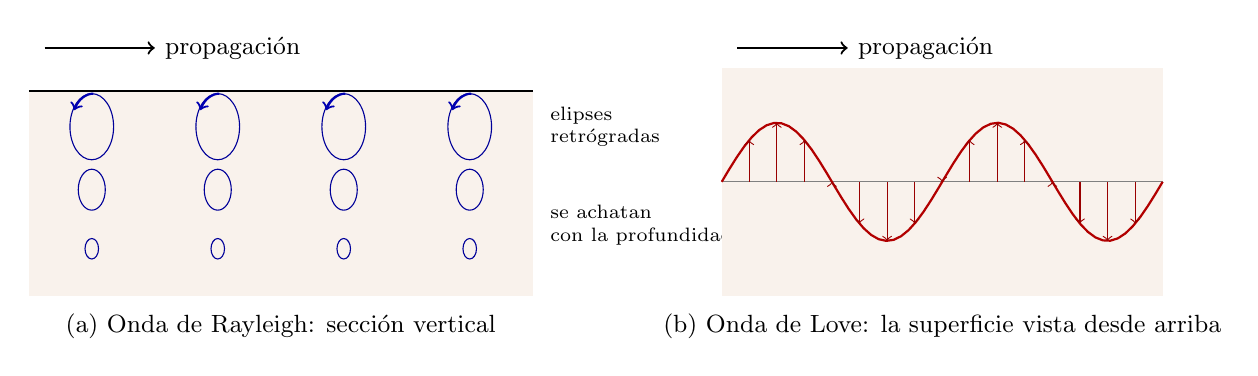
\begin{tikzpicture}[font=\small, x=1cm, y=1cm]
% Rayleigh: vertical section
\fill[brown!10] (0,0) rectangle (6.4,-2.6);
\draw[thick] (0,0) -- (6.4,0);
\draw[->, thick] (0.2,0.55) -- (1.6,0.55) node[right] {propagación};
\foreach \x/\s in {0.8/1, 2.4/-1, 4.0/1, 5.6/-1} {
  \foreach \z/\a in {-0.45/0.42, -1.25/0.26, -2.0/0.13} {
    \draw[blue!60!black] (\x,\z) ellipse ({0.66*\a} and {\a});
  }
}
\foreach \x in {0.8, 2.4, 4.0, 5.6} {
  \draw[->, blue!70!black, thick] (\x+0.02,-0.03) arc (90:150:{0.28} and {0.42});
}
\node[anchor=north] at (3.2,-2.7) {(a) Onda de Rayleigh: sección vertical};
\node[anchor=west, font=\scriptsize, align=left] at (6.5,-0.45) {elipses\\ retrógradas};
\node[anchor=west, font=\scriptsize, align=left] at (6.5,-1.7) {se achatan\\con la profundidad};
% Love: plan view of the surface
\begin{scope}[xshift=8.8cm]
\fill[brown!10] (0,0.3) rectangle (5.6,-2.6);
\draw[->, thick] (0.2,0.55) -- (1.6,0.55) node[right] {propagación};
\draw[gray, thin] (0,-1.15) -- (5.6,-1.15);
\draw[red!70!black, thick, domain=0:5.6, samples=60] plot (\x,{-1.15+0.75*sin(\x*360/2.8)});
\foreach \x in {0.35,0.7,...,5.3} {
  \pgfmathsetmacro{\d}{0.75*sin(\x*360/2.8)}
  \draw[->, red!60!black] (\x,-1.15) -- (\x,{-1.15+\d});
}
\node[anchor=north] at (2.8,-2.7) {(b) Onda de Love: la superficie vista desde arriba};
\end{scope}
\end{tikzpicture}

\par\smallskip{\small Movimientos de partícula de las dos ondas superficiales (esquemático).
(a) Una \omterm{def:b3:seismology-imaging:surface-waves}{onda de Rayleigh} mueve el terreno en el plano vertical de propagación,
según elipses que se invierten hacia atrás en la parte superior (retrógradas) cerca de la superficie y
se reducen con la profundidad. (b) Una \omterm{def:b3:seismology-imaging:surface-waves}{onda de Love} mueve el terreno horizontalmente, perpendicularmente a la
dirección de propagación: las flechas muestran el desplazamiento en un instante
a lo largo de una línea de la superficie.}
\label{fig:b3:seismology-imaging:particle-motion}
\end{omfigure}

\begin{theorem}[Dispersión de las ondas de Love en una capa sobre un semiespacio]\label{thm:b3:seismology-imaging:love}
Una capa de espesor $H$, módulo de cizalla $\mu_1$ y velocidad S $\beta_1$ descansa sobre un
semiespacio de módulo de cizalla $\mu_2$ y velocidad S $\beta_2 > \beta_1$. Una
\omterm{def:b3:seismology-imaging:surface-waves}{onda de Love} de frecuencia angular $\omega$ y número de onda $k$ se propaga con la
velocidad de fase $c = \omega/k$, $\beta_1 < c < \beta_2$, si y solo si
\[
  \tan\!\left(kH q_1\right) = \frac{\mu_2 q_2}{\mu_1 q_1},
  \qquad q_1 = \sqrt{\frac{c^2}{\beta_1^2} - 1},\quad
  q_2 = \sqrt{1 - \frac{c^2}{\beta_2^2}} .
\]
El modo fundamental es la raíz con $0 < kHq_1 < \pi/2$; los sobretonos tienen
$kHq_1$ en $(n\pi, n\pi + \pi/2)$.
\end{theorem}

\begin{proof}
Tómese $x$ en la dirección de propagación, $y$ horizontal y perpendicular a ella, y $z$ hacia abajo desde
la superficie libre, y búsquese un desplazamiento
$u_y = f(z)\,e^{i(kx - \omega t)}$, siendo nulas las demás componentes. Cada capa
obedece a la ecuación de ondas $\partial^2 u_y/\partial t^2 = \beta^2\nabla^2 u_y$, de modo que
$f'' = -k^2\left(c^2/\beta^2 - 1\right) f$. En la capa, $c > \beta_1$, y
$f = A\cos(kq_1z) + B\sin(kq_1z)$. En el semiespacio, $c < \beta_2$, y la
solución que permanece acotada en profundidad es $f = C\,e^{-kq_2(z - H)}$.
La tracción de cizalla sobre un plano horizontal es $\mu\,\partial u_y/\partial z$.
En la superficie libre se anula: $f'(0) = 0$, luego $B = 0$. En $z = H$ el
desplazamiento y la tracción son continuos:
\[
  A\cos(kq_1H) = C, \qquad -\mu_1 A\,kq_1\sin(kq_1H) = -\mu_2\,kq_2\,C .
\]
Dividiendo la segunda ecuación entre la primera se obtiene el resultado. Como el
lado derecho es positivo, $kHq_1$ se encuentra en un cuarto de periodo en el que la
tangente es positiva; el intervalo más pequeño de este tipo da el modo fundamental.
\end{proof}

Para un periodo dado la ecuación se resuelve para $c$ por bisección; la velocidad de grupo
se obtiene de $U = \mathrm d\omega/\mathrm dk$. A periodos cortos
($kH$ grande) la raíz está cerca de $c = \beta_1$: la onda vive en la capa. A
periodos largos ($kH \to 0$) debe cumplirse $kHq_1 \to 0$ con el lado derecho
también pequeño, lo que obliga a $c \to \beta_2$: la onda llega hasta el interior del
semiespacio y viaja a su velocidad. Entre ambos extremos, la velocidad de fase
aumenta de forma constante con el periodo.

\begin{definition}[Dispersión de las ondas superficiales]\label{def:b3:seismology-imaging:dispersion}
La \emph{dispersión de las ondas superficiales}\index{dispersión de las ondas superficiales} es la dependencia
de las velocidades de fase y de grupo de una \omterm{def:b3:seismology-imaging:surface-waves}{onda de Rayleigh} o de Love respecto de su periodo. En
una Tierra estratificada surge porque una onda de periodo más largo alcanza mayor profundidad
(aproximadamente un tercio de una longitud de onda para el modo fundamental) y promedia
roca más rápida; las curvas de dispersión $c(T)$ y $U(T)$ medidas entre un terremoto
y una estación, o entre dos estaciones, se invierten para obtener la velocidad S en
función de la profundidad.
\end{definition}

\begin{omfigure}
\begin{tikzpicture}
\begin{axis}[omrecord, xmode=log, width=0.82\linewidth, height=0.5\linewidth,
  xmin=3, xmax=150, ymin=3.3, ymax=4.6, log basis x=10,
  xtick={3,5,10,20,50,100,150}, xticklabels={3,5,10,20,50,100,150},
  xlabel={periodo $T$ (\unit{s})}, ylabel={velocidad (\unit{km.s^{-1}})},
  legend style={at={(0.03,0.62)}, anchor=west}, legend cell align=left]
\addplot[blue!70!black, thick] table[x=period, y=c] {figdata/out/bachelor-3-love_dispersion-curve.dat};
\addlegendentry{velocidad de fase $c$}
\addplot[red!70!black, thick] table[x=period, y=U] {figdata/out/bachelor-3-love_dispersion-curve.dat};
\addlegendentry{velocidad de grupo $U$}
\draw[gray, dashed] (axis cs:3,3.5) -- (axis cs:150,3.5);
\draw[gray, dashed] (axis cs:3,4.5) -- (axis cs:150,4.5);
\node[font=\scriptsize, anchor=south] at (axis cs:80,3.5) {$\beta_1 = 3.5$};
\node[font=\scriptsize, anchor=south west] at (axis cs:3.1,4.5) {$\beta_2 = 4.5$};
\addplot[only marks, mark=*, mark size=1.4pt, red!70!black] coordinates {(19.2,3.384)};
\node[font=\scriptsize, anchor=south, red!70!black] at (axis cs:19.2,3.39) {fase de Airy};
\end{axis}
\end{tikzpicture}

\par\smallskip{\small \omterm{def:b3:seismology-imaging:surface-waves}{Ondas de Love} fundamentales en una capa de \qty{35}{km}
($\beta_1 = \qty{3.5}{km.s^{-1}}$, \qty{2.7}{g.cm^{-3}}) sobre un semiespacio
($\beta_2 = \qty{4.5}{km.s^{-1}}$, \qty{3.3}{g.cm^{-3}}), un modelo simplificado de
corteza continental sobre el manto, calculadas a partir del
\cref{thm:b3:seismology-imaging:love}. La velocidad de fase sube desde la
velocidad S de la capa hasta la del semiespacio; la velocidad de grupo es menor y tiene un
mínimo, \qty{3.384}{km.s^{-1}} a \qty{19.2}{s}, donde las ondas de periodos vecinos
llegan juntas como un gran pulso tardío (la fase de Airy).}
\label{fig:b3:seismology-imaging:love}
\end{omfigure}

En este modelo la velocidad de fase a \qty{20}{s} es \qty{3.79}{km.s^{-1}} y a
\qty{100}{s} \qty{4.444}{km.s^{-1}}; las velocidades de grupo son 3.384 y
\qty{4.333}{km.s^{-1}}. En un sismograma registrado a unos pocos miles de kilómetros
de distancia, los periodos largos llegan primero y las ondas de 20~s, al final, de
modo que el tren de ondas se extiende en una oscilación larga que se acorta
lentamente. Medir la velocidad de grupo a muchos periodos y en muchas trayectorias
da mapas del espesor de la corteza y del manto superior, independientes de los
tiempos de recorrido de las ondas de cuerpo.

\section{La Tierra resuena: modos normales}

Una onda superficial de periodo muy largo tiene una longitud de onda comparable al
radio terrestre; da la vuelta al globo y se encuentra consigo misma. Las ondas que
interfieren constructivamente son las ondas estacionarias de toda la esfera, sus
modos normales, y tras un gran terremoto son la última señal que se extingue.
Su teoría, un problema de valores propios para la Tierra elástica y autogravitante,
queda fuera de este capítulo; su descripción, no.

Los modos de una Tierra con simetría esférica forman dos familias. En los modos
\emph{toroidales}, ${}_nT_\ell$, el movimiento es horizontal, una torsión de
capas esféricas unas contra otras, sin cambio de radio ni de volumen: son
las ondas estacionarias de las \omterm{def:b3:seismology-imaging:surface-waves}{ondas de Love}. En los modos \emph{esferoidales}, 
${}_nS_\ell$, el movimiento tiene componentes radial y horizontal, y la Tierra cambia
de forma: son las ondas estacionarias de las \omterm{def:b3:seismology-imaging:surface-waves}{ondas de Rayleigh}, acopladas a las ondas
de cuerpo y a la gravedad. El índice $\ell$ es el grado angular, el número de líneas
nodales del patrón en la superficie; $n$ cuenta los nodos del movimiento con el radio,
con $n = 0$ para el modo fundamental. El modo esferoidal más grave, ${}_0S_2$, estira
la Tierra alternativamente en un esferoide prolato y en uno oblato; el modo toroidal
más grave, ${}_0T_2$, retuerce los hemisferios norte y sur en sentidos
opuestos. Sus periodos observados son:
\begin{center}
\small
% ledger: seis5:modes-T, seis5:modes-S
\begin{tabular}{lcccc}
\hline
modo & ${}_0T_2$ & ${}_1T_2$ & ${}_0T_3$ & ${}_1T_3$ \\
periodo (\unit{min}) & 44.01 & 12.61 & 28.43 & 11.59 \\
\hline
modo & ${}_0S_2$ & ${}_1S_2$ & ${}_0S_3$ & ${}_1S_3$ \\
periodo (\unit{min}) & 53.89 & 24.51 & 35.56 & 17.68 \\
\hline
\end{tabular}
\end{center}
Cada periodo es un promedio sobre todo el planeta de sus módulos elásticos y de su
densidad, ponderado según las zonas donde se desplaza el modo: los modos toroidales solo perciben el
manto sólido y la corteza, y los esferoidales también el núcleo. Ajustar los
periodos de centenares de modos es la única forma sismológica de pesar el
interior: restringe la densidad, no solo las velocidades, y PREM se construyó para ajustarlos
en conjunto con los tiempos de recorrido. La rotación y la elipticidad de la Tierra
desdoblan cada modo de grado $\ell$ en $2\ell + 1$ frecuencias ligeramente distintas,
el análogo del efecto Zeeman.

\begin{history}[La Tierra después del terremoto chileno]
El terremoto chileno de 1960 fue registrado por sismómetros pendulares de periodo largo
y por deformímetros, instrumentos que miden el cambio de longitud de una
barra o un hilo horizontal largo anclado en la roca. El análisis espectral de unos pocos días de
registro mostró picos nítidos en los periodos previstos de los modos más graves: toda
la Tierra había entrado en resonancia, y se cumplieron las predicciones de la teoría
elástica de una Tierra esférica y autogravitante. El registro del deformímetro
de Isabella, en California, fue analizado de nuevo en 1978 con métodos más modernos:
mostró con claridad el desdoblamiento de ${}_0T_3$, ${}_0T_4$, ${}_0S_4$
y ${}_0S_5$ por la rotación y la elipticidad de la Tierra, y confirmó el de
${}_0S_2$ y ${}_0S_3$.
% ledger: stein78:chile-modes, usgs5:chile1960
La sismología de modos normales, nacida de un solo terremoto, utiliza hoy las redes de
estaciones de banda muy ancha que registran cada gran terremoto.
\end{history}

\section{Problemas lineales inversos}\label{sec:b3:seismology-imaging:inverse}

Todos los métodos de este capítulo hasta ahora calculan datos a partir de un modelo. La
tarea de la obtención de imágenes es la inversa.

\begin{definition}[Problema directo, problema inverso]\label{def:b3:seismology-imaging:inverse}
Sea un modelo de la Tierra descrito por un vector $\mathbf m$ de $M$ parámetros
y las observaciones por un vector $\mathbf d$ de $N$ datos. El \emph{problema
directo}\index{problema directo} consiste en calcular los datos $\mathbf d = g(\mathbf m)$
que produciría un modelo dado, mediante una teoría física. El \emph{problema
inverso}\index{problema inverso} consiste en estimar el modelo a partir de datos que
llevan errores, $\mathbf d = g(\mathbf m) + \mathbf e$, y en indicar con qué precisión
queda determinada cada parte del modelo. El problema es lineal cuando $g(\mathbf m) =
\mathsf G\mathbf m$ para una matriz fija $N\times M$ $\mathsf G$, el núcleo.
\end{definition}

Ajustar una recta a tiempos de recorrido es un problema lineal inverso con
$M = 2$ (ejercicio 7); una tomografía de tiempos de recorrido es una con miles de
parámetros. Se presentan tres casos. Si $N > M$ y los datos restringen cada
parámetro, el problema está \emph{sobredeterminado}: ningún modelo ajusta cada dato
exactamente, y la mejor solución se busca en sentido estadístico. Si alguna combinación de
parámetros deja los datos sin cambios ($\mathsf G\mathbf m_0 = \mathbf 0$ para
algún $\mathbf m_0 \ne \mathbf 0$), el problema está \emph{infradeterminado} en esa
dirección, y ninguna cantidad de datos de ese tipo lo corregirá. Los problemas reales son
mixtos: sobredeterminados en unas partes del modelo e infradeterminados en
otras.

\begin{theorem}[Estimación por mínimos cuadrados ponderados]\label{thm:b3:seismology-imaging:wls}
Sea $\mathbf d = \mathsf G\mathbf m + \mathbf e$, donde los errores $\mathbf e$
tienen media cero y la matriz de covarianza $\mathsf C_d$ (diagonal
$\sigma_i^2$ para errores independientes). Si la matriz
$\mathsf N = \mathsf G^{\mathsf T}\mathsf C_d^{-1}\mathsf G$ es invertible, el
modelo que minimiza el desajuste
\[
  \chi^2(\mathbf m) = (\mathbf d - \mathsf G\mathbf m)^{\mathsf T}\mathsf C_d^{-1}
  (\mathbf d - \mathsf G\mathbf m)
\]
es la \emph{estimación por mínimos cuadrados ponderados}\index{estimación por mínimos cuadrados ponderados}
\[
  \hat{\mathbf m} = \mathsf N^{-1}\mathsf G^{\mathsf T}\mathsf C_d^{-1}\mathbf d ,
\]
es insesgada, y su matriz de covarianza es
$\mathsf C_{\hat m} = \mathsf N^{-1}$.
\end{theorem}

\begin{proof}
$\chi^2$ es una función cuadrática de $\mathbf m$ con gradiente
$-2\mathsf G^{\mathsf T}\mathsf C_d^{-1}(\mathbf d - \mathsf G\mathbf m)$, que
se anula en las ecuaciones normales $\mathsf N\mathbf m = \mathsf G^{\mathsf T}
\mathsf C_d^{-1}\mathbf d$; la matriz hessiana $2\mathsf N$ es definida positiva cuando
$\mathsf N$ es invertible (entonces $\mathbf x^{\mathsf T}\mathsf N\mathbf x =
\|\mathsf C_d^{-1/2}\mathsf G\mathbf x\|^2 > 0$ para $\mathbf x \ne 0$), de modo que el
punto estacionario es el mínimo. Se escribe $\hat{\mathbf m} = \mathsf H\mathbf d$ con
$\mathsf H = \mathsf N^{-1}\mathsf G^{\mathsf T}\mathsf C_d^{-1}$. Entonces
$\mathsf H\mathsf G = \mathsf I$, así que $\hat{\mathbf m} = \mathbf m + \mathsf H\mathbf e$
tiene valor medio $\mathbf m$, y su covarianza es
$\mathsf H\mathsf C_d\mathsf H^{\mathsf T} =
\mathsf N^{-1}\mathsf G^{\mathsf T}\mathsf C_d^{-1}\mathsf C_d\mathsf C_d^{-1}
\mathsf G\mathsf N^{-1} = \mathsf N^{-1}$.
\end{proof}

Los pesos hacen lo que pide la intuición: un dato con la mitad de error cuenta
cuatro veces más. La matriz de covarianza da a cada parámetro su error típico
$\sqrt{(\mathsf N^{-1})_{jj}}$ y las correlaciones entre ellos. Si el modelo
es correcto y los errores son gaussianos, el $\chi^2$ mínimo sigue una ley de
$\chi^2$ con $N - M$ grados de libertad: un valor muy superior a $N - M$ indica que
los errores se subestimaron o que el modelo es demasiado simple; muy inferior, que
los errores se sobreestimaron.

Cuando $\mathsf N$ es singular o casi singular, la estimación no existe o está
dominada por el ruido amplificado en las direcciones mal restringidas. El
remedio habitual es buscar un modelo que ajuste razonablemente los datos y que no
sea innecesariamente grande.

\begin{definition}[Mínimos cuadrados amortiguados, curva de compromiso]\label{def:b3:seismology-imaging:damped}
Para un parámetro de amortiguamiento $\varepsilon > 0$, la \emph{estimación por
mínimos cuadrados amortiguados}\index{mínimos cuadrados amortiguados} es el modelo que minimiza
\[
  \Phi_\varepsilon(\mathbf m) = \chi^2(\mathbf m) + \varepsilon^2\|\mathbf m\|^2 ,
  \qquad
  \mathbf m_\varepsilon = \left(\mathsf N + \varepsilon^2\mathsf I\right)^{-1}
  \mathsf G^{\mathsf T}\mathsf C_d^{-1}\mathbf d .
\]
La \emph{curva de compromiso}\index{curva de compromiso} es la curva que se traza al variar
$\varepsilon$, el par (tamaño del modelo $\|\mathbf m_\varepsilon\|$,
desajuste $\chi^2(\mathbf m_\varepsilon)$): un amortiguamiento pequeño ajusta los datos de cerca
con un modelo grande y rugoso; un amortiguamiento grande da un modelo pequeño y un ajuste pobre.
\end{definition}

La fórmula se obtiene como en el \cref{thm:b3:seismology-imaging:wls}: el gradiente
de $\Phi_\varepsilon$ es $-2\mathsf G^{\mathsf T}\mathsf C_d^{-1}(\mathbf d -
\mathsf G\mathbf m) + 2\varepsilon^2\mathbf m$, y $\mathsf N + \varepsilon^2
\mathsf I$ es siempre invertible, ya que sus autovalores son los de
$\mathsf N$ (todos $\ge 0$) aumentados en $\varepsilon^2$. El amortiguamiento suele
elegirse cerca del codo de la \omterm{def:b3:seismology-imaging:damped}{curva de compromiso}, o de modo que $\chi^2$ sea aproximadamente
el número de datos, el desajuste que cabe esperar solo por los errores. El precio es que la
estimación deja de ser insesgada.

\begin{definition}[Matriz de resolución del modelo]\label{def:b3:seismology-imaging:resolution}
Para una estimación lineal $\mathbf m_\varepsilon = \mathsf H_\varepsilon \mathbf d$
del modelo $\mathbf m$ a partir de los datos $\mathbf d = \mathsf G\mathbf m + \mathbf e$,
la \emph{matriz de resolución del modelo}\index{matriz de resolución del modelo} es
$\mathsf R = \mathsf H_\varepsilon\mathsf G$, de modo que
\[
  \mathbf m_\varepsilon = \mathsf R\,\mathbf m + \mathsf H_\varepsilon\mathbf e .
\]
Para \omterm{def:b3:seismology-imaging:damped}{mínimos cuadrados amortiguados}, $\mathsf R = (\mathsf N + \varepsilon^2\mathsf I)^{-1}
\mathsf N$. La fila $j$ de $\mathsf R$ muestra cómo la estimación del parámetro $j$
promedia los parámetros verdaderos; $\mathsf R = \mathsf I$ significa resolución perfecta.
\end{definition}

Si $\mathsf N$ tiene los autovectores ortonormales $\mathbf u_k$ y los autovalores
$\lambda_k$, entonces $\mathsf R = \sum_k \frac{\lambda_k}{\lambda_k + \varepsilon^2}
\mathbf u_k\mathbf u_k^{\mathsf T}$: las direcciones que los datos restringen bien
($\lambda_k \gg \varepsilon^2$) pasan casi sin cambios, mientras que las que restringen
mal quedan suprimidas. La traza de $\mathsf R$ cuenta los parámetros que los datos
resuelven efectivamente, y la covarianza de la estimación,
$\mathsf H_\varepsilon\mathsf C_d\mathsf H_\varepsilon^{\mathsf T}$, se reduce a medida que
disminuye la resolución: el amortiguamiento intercambia resolución por estabilidad.

\begin{omfigure}
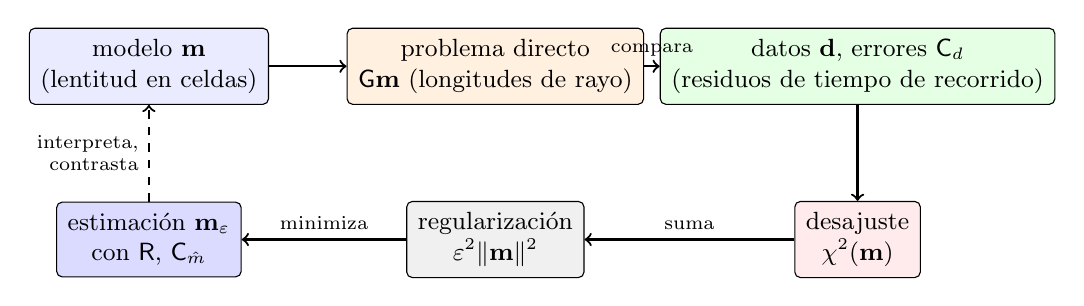
\begin{tikzpicture}[font=\small, node distance=0.5cm,
  box/.style={draw, rounded corners=2pt, fill=#1, minimum height=0.9cm, align=center, inner sep=4pt},
  box/.default=gray!8]
\node[box=blue!8] (m) at (0,0) {modelo $\mathbf m$\\(lentitud en celdas)};
\node[box=orange!12] (g) at (4.4,0) {problema directo\\$\mathsf G\mathbf m$ (longitudes de rayo)};
\node[box=green!10] (d) at (9.0,0) {datos $\mathbf d$, errores $\mathsf C_d$\\(residuos de tiempo de recorrido)};
\node[box=red!8] (mis) at (9.0,-2.2) {desajuste\\$\chi^2(\mathbf m)$};
\node[box=gray!12] (reg) at (4.4,-2.2) {regularización\\$\varepsilon^2\|\mathbf m\|^2$};
\node[box=blue!14] (est) at (0,-2.2) {estimación $\mathbf m_\varepsilon$\\con $\mathsf R$, $\mathsf C_{\hat m}$};
\draw[->, thick] (m) -- (g);
\draw[->, thick] (g) -- node[above, font=\scriptsize] {compara} (d);
\draw[->, thick] (d) -- (mis);
\draw[->, thick] (mis) -- node[above, font=\scriptsize] {suma} (reg);
\draw[->, thick] (reg) -- node[above, font=\scriptsize] {minimiza} (est);
\draw[->, thick, dashed] (est) -- node[left, font=\scriptsize, align=right] {interpreta,\\contrasta} (m);
\end{tikzpicture}

\par\smallskip{\small El \omterm{def:b3:seismology-imaging:inverse}{problema inverso} lineal como un bucle (esquema). El
\omterm{def:b3:seismology-imaging:inverse}{problema directo} predice datos a partir de un modelo; el desajuste, ponderado por los
errores de los datos, mide la discrepancia; el término de regularización mantiene el modelo
pequeño; minimizar su suma da la estimación, que solo es interpretable
junto con su matriz de resolución y su covarianza.}
\label{fig:b3:seismology-imaging:inverse-loop}
\end{omfigure}

\section{Tomografía sísmica}\label{sec:b3:seismology-imaging:tomography}

\begin{definition}[Tomografía sísmica, residuo de tiempo de recorrido]\label{def:b3:seismology-imaging:tomography}
El \emph{residuo de tiempo de recorrido}\index{residuo de tiempo de recorrido} de una llegada es el
tiempo de recorrido observado menos el tiempo predicho por un modelo de referencia,
$\delta t = T_{\text{obs}} - T_{\text{ref}}$, tras corregir la localización del
foco y el tiempo origen, la elevación de la estación y la
elipticidad de la Tierra. La \emph{tomografía sísmica}\index{tomografía sísmica} es la
estimación de las desviaciones tridimensionales de las velocidades sísmicas respecto de
un modelo de referencia, $\delta v(\mathbf x)$, a partir de un conjunto grande de residuos (o de
formas de onda), resolviendo un \omterm{def:b3:seismology-imaging:inverse}{problema inverso}.
\end{definition}

Se escribe $s = 1/v$ para la lentitud. El tiempo de recorrido a lo largo de un rayo $\Gamma$ es
$T = \int_\Gamma s\,\mathrm dl$; pero el propio rayo depende de las velocidades,
lo que parece volver el problema no lineal. La respuesta de primer orden es que
eso no importa.

\begin{proposition}[Residuo de tiempo de recorrido linealizado]\label{prop:b3:seismology-imaging:linear}
Si la lentitud del modelo de referencia $s_0$ se perturba hasta $s_0 + \delta s$,
el tiempo de recorrido entre dos puntos fijos cambia, a primer orden en
$\delta s$, en
\[
  \delta t = \int_{\Gamma_0}\delta s\,\mathrm dl ,
\]
siendo la integral tomada a lo largo del rayo $\Gamma_0$ del modelo de referencia; la
anomalía relativa de velocidad es $\delta v/v_0 = -\delta s/s_0$ al mismo orden.
\end{proposition}

\begin{proof}
Por el principio de Fermat, el rayo $\Gamma_0$ hace que el tiempo de recorrido
$\int s_0\,\mathrm dl$ sea estacionario frente a trayectorias vecinas: al desplazar la trayectoria una
pequeña cantidad $\epsilon$, el tiempo cambia en un término de orden $\epsilon^2$ únicamente.
El nuevo rayo $\Gamma$ difiere de $\Gamma_0$ en una cantidad del orden de $\delta s$;
por tanto $\int_\Gamma(s_0 + \delta s)\,\mathrm dl = \int_{\Gamma_0}s_0\,\mathrm dl +
O(\delta s^2) + \int_{\Gamma_0}\delta s\,\mathrm dl + O(\delta s^2)$. Finalmente
$\delta(1/s) = -\delta s/s_0^2$, por lo que $\delta v/v_0 = -\delta s/s_0$.
\end{proof}

Se divide la región en $M$ celdas de perturbación uniforme de lentitud $\delta s_j$.
El residuo del rayo $i$ pasa a ser $\delta t_i = \sum_j L_{ij}\,\delta s_j$, donde
$L_{ij}$ es la longitud del rayo de referencia $i$ en la celda $j$: un \omterm{def:b3:seismology-imaging:inverse}{problema inverso} lineal
cuyo núcleo es la matriz de longitudes de rayo, casi todas cuyas entradas
son nulas. Los residuos son pequeños: en un manto a
\qty{8}{km.s^{-1}}, una región de \qty{200}{km} de anchura con una velocidad \qty{3}{\percent}
mayor adelanta un rayo vertical unos \qty{0.7}{s} (ejercicio 9).

\begin{method}[Tomografía de tiempos de recorrido]\label{met:b3:seismology-imaging:tomo}
\begin{enumerate}
  \item Se toman los tiempos de llegada de una fase (por ejemplo, P) en todas las estaciones, para
        terremotos cuya localización es bien conocida; se calculan los residuos
        frente a una \omterm{def:b3:seismology-imaging:tables}{tabla de tiempos de recorrido}, corregidos por elipticidad y por la
        elevación de la estación.
  \item Se trazan los rayos de referencia y se divide la región en celdas (o se desarrolla
        $\delta s$ en funciones suaves); se rellena la matriz de longitudes de rayo.
  \item Se asigna a cada residuo su error, a partir de la precisión de la lectura, y se resuelve
        el problema de \omterm{def:b3:seismology-imaging:damped}{mínimos cuadrados amortiguados} para un intervalo de valores de amortiguamiento; se dibuja
        la \omterm{def:b3:seismology-imaging:damped}{curva de compromiso} y se elige el amortiguamiento cerca de su codo.
  \item Se comprueba la resolución: se calculan los residuos que un modelo sintético conocido
        produciría a través de los mismos rayos, se añade ruido y se invierten
        con el mismo amortiguamiento, y se comparan los resultados.
  \item Se interpretan únicamente las anomalías que la prueba muestra que los rayos pueden
        recuperar, entendiendo sus amplitudes como cotas inferiores.
\end{enumerate}
\end{method}

\begin{definition}[Prueba del tablero de ajedrez]\label{def:b3:seismology-imaging:checkerboard}
Una \emph{prueba del tablero de ajedrez}\index{prueba del tablero de ajedrez} es una prueba de resolución en
la que el modelo sintético es un patrón regular de celdas alternativamente rápidas y lentas:
los residuos sintéticos calculados a través de la geometría real de los rayos, con ruido
de magnitud similar a los errores reales, se invierten con la misma parametrización y
amortiguamiento. Donde se recupera el patrón, pueden resolverse estructuras de ese tamaño;
donde aparece difuminado o se pierde, no pueden.
\end{definition}

Las figuras siguientes aplican la prueba a una sección de modelo de \qty{800}{km} de anchura y
\qty{400}{km} de profundidad, dividida en 128 celdas de \qty{50}{km}. Veinte focos se sitúan
a lo largo de su base y treinta y dos estaciones a lo largo de su parte superior, y solo se usan los rayos dentro de
\ang{45} de la vertical: 480 rayos que todos ascienden casi verticalmente,
la geometría de los rayos de terremotos lejanos que ascienden bajo una red. El
modelo sintético tiene bloques de $2\times2$ celdas, \qty{3}{\percent} más rápidos o más lentos
alrededor de \qty{8}{km.s^{-1}}; los residuos llevan ruido gaussiano de
\qty{0.05}{s}.
% figdata: tomo_checkerboard.py (invented geometry; no real data)

\begin{omfigure}
\begin{tikzpicture}
\begin{groupplot}[group style={group size=2 by 2, horizontal sep=0.9cm, vertical sep=1.25cm},
  width=0.46\linewidth, height=0.3\linewidth, xmin=0, xmax=800, ymin=0, ymax=400,
  axis on top, enlargelimits=false, tick label style={font=\scriptsize},
  title style={font=\small, yshift=-1ex},
  colormap={tomo}{rgb255(0cm)=(178,24,43); rgb255(1cm)=(244,165,130); rgb255(2cm)=(247,247,247); rgb255(3cm)=(146,197,222); rgb255(4cm)=(33,102,172)},
  point meta min=-4, point meta max=4]
\nextgroupplot[title={(a) modelo sintético}, ylabel={\scriptsize altura (km)}]
\addplot[matrix plot*, mesh/cols=16, point meta=explicit] table[x=x, y=y, meta=dv] {figdata/out/bachelor-3-tomo_checkerboard-true.dat};
\nextgroupplot[title={(b) muestra de los 480 rayos}, colormap/blackwhite]
\addplot[gray!70!black, thin, unbounded coords=jump] table[x=x, y=y] {figdata/out/bachelor-3-tomo_checkerboard-rays.dat};
\addplot[only marks, mark=triangle*, mark size=1.6pt, black, clip=false] table[x=x, y=y] {figdata/out/bachelor-3-tomo_checkerboard-receivers.dat};
\addplot[only marks, mark=star, mark size=1.8pt, red!70!black, clip=false] table[x=x, y=y] {figdata/out/bachelor-3-tomo_checkerboard-sources.dat};
\nextgroupplot[title={(c) recuperado, $\varepsilon = \qty{3}{km}$}, ylabel={\scriptsize altura (km)}, xlabel={\scriptsize distancia (km)}]
\addplot[matrix plot*, mesh/cols=16, point meta=explicit] table[x=x, y=y, meta=dv] {figdata/out/bachelor-3-tomo_checkerboard-rec-low.dat};
\nextgroupplot[title={(d) recuperado, $\varepsilon = \qty{60}{km}$}, xlabel={\scriptsize distancia (km)},
  colorbar right, colorbar style={width=0.2cm, ytick={-4,-2,0,2,4}, ylabel={\scriptsize $\delta v/v$ (\%)}, tick label style={font=\scriptsize}}]
\addplot[matrix plot*, mesh/cols=16, point meta=explicit] table[x=x, y=y, meta=dv] {figdata/out/bachelor-3-tomo_checkerboard-rec-high.dat};
\end{groupplot}
\end{tikzpicture}

\par\smallskip{\small Una \omterm{def:b3:seismology-imaging:checkerboard}{prueba del tablero de ajedrez} (geometría inventada). (a) El
modelo sintético: bloques de \qty{100}{km} de anchura, \qty{3}{\percent} más rápidos (azul) o
más lentos (rojo). (b) Los 20 focos (estrellas), las 32
estaciones (triángulos) y algunos de los rayos, todos dentro de \ang{45} de la vertical. (c) Con
amortiguamiento ligero se recuperan los bloques, aunque con ruido, con anomalías de hasta unos
\qty{8}{\percent} allí donde cruzan pocos rayos (los colores se saturan en
\qty{4}{\percent}). (d) Con amortiguamiento fuerte el patrón es nítido, pero su
amplitud queda reducida, sobre todo a lo largo de los bordes laterales, donde cruzan pocos rayos
y todos con ángulos similares.}
\label{fig:b3:seismology-imaging:checkerboard}
\end{omfigure}

\begin{omfigure}
\begin{tikzpicture}
\begin{axis}[omrecord, width=0.62\linewidth, height=0.42\linewidth,
  xlabel={norma del modelo $\|\delta v/v\|$ (\unit{\percent})},
  ylabel={desajuste $\|\mathsf G\mathbf m - \mathbf d\|$ (\unit{s})}, xmin=0, xmax=42, ymin=0, ymax=12]
\addplot[blue!70!black, thick] table[x=norm, y=misfit] {figdata/out/bachelor-3-tomo_checkerboard-tradeoff.dat};
\addplot[only marks, mark=*, mark size=1.8pt, red!70!black] coordinates {(38.84,0.862) (29.42,1.159)};
\node[font=\scriptsize, anchor=south, red!70!black] at (axis cs:38.84,1.3) {$\varepsilon = 3$};
\node[font=\scriptsize, anchor=east, red!70!black] at (axis cs:28.6,0.55) {$\varepsilon = 60$};
\draw[gray, dashed] (axis cs:0,1.095) -- (axis cs:42,1.095);
\node[font=\scriptsize, anchor=south west] at (axis cs:1,1.15) {esperado a partir del ruido};
\draw[green!45!black, densely dotted] (axis cs:33.94,0) -- (axis cs:33.94,12);
\node[font=\scriptsize, anchor=north west, green!45!black] at (axis cs:34.2,11.8) {modelo verdadero};
\node[font=\scriptsize, anchor=west] at (axis cs:14,10.5) {amortiguamiento fuerte};
\node[font=\scriptsize, anchor=east] at (axis cs:41,3.2) {amortiguamiento ligero};
\end{axis}
\end{tikzpicture}

\par\smallskip{\small La \omterm{def:b3:seismology-imaging:damped}{curva de compromiso} de la \omterm{def:b3:seismology-imaging:checkerboard}{prueba del tablero de ajedrez}, para valores de amortiguamiento
$\varepsilon$ desde 0.1 hasta \qty{1000}{km} (el núcleo se expresa en kilómetros,
con errores iguales). A lo largo de la parte plana, más amortiguamiento apenas cuesta ajuste: el
modelo se contrae al perder ruido. El codo se sitúa donde el desajuste sube por encima del
nivel esperado a partir del ruido por sí solo, $\sigma\sqrt{480} = \qty{1.095}{s}$; los
dos modelos amortiguados de la figura anterior quedan a ambos lados de él, y la
norma del tablero de ajedrez verdadero, \qty{33.9}{\percent}, queda entre ambos. Más allá del
codo, el amortiguamiento elimina estructura que los datos requieren.}
\label{fig:b3:seismology-imaging:tradeoff}
\end{omfigure}

La prueba ilustra los tres límites de toda imagen tomográfica. La resolución
viene fijada por los rayos: donde todos los rayos son paralelos, una anomalía se extiende a lo largo de ellos,
y una celda atravesada por pocos rayos apenas queda restringida. El amortiguamiento reduce las
amplitudes: las anomalías recuperadas son cotas inferiores.
Además, la imagen depende del modelo de referencia y de la parametrización: solo se
representan las desviaciones respecto de la referencia, y nada menor que una celda.
Con estas cautelas, las imágenes globales de ondas P y S muestran las losas del
volumen de primer año (en su capítulo sobre subducción) como regiones rápidas tabulares que descienden
desde las fosas, algunas aplanándose sobre la discontinuidad de 670 km, otras
hundiéndose en el manto inferior; y amplias regiones lentas bajo el Pacífico y
África sobre el núcleo, con conductos lentos más estrechos bajo algunos puntos calientes, que son los candidatos
a plumas del manto del mismo volumen.

\begin{inthefield}[Una estación de banda ancha y un despliegue de fondo oceánico]
\begin{minipage}[t]{0.55\linewidth}\vspace{0pt}
Una estación permanente de banda ancha es un lugar tranquilo: el sismómetro se apoya sobre un
pilar de hormigón anclado al lecho rocoso, en una cámara enterrada o en un túnel corto, bajo un
escudo térmico, porque una corriente de aire o un cambio de unas pocas centésimas de grado
inclina el instrumento más que un terremoto lejano. Sus tres componentes,
vertical, norte y este, se digitalizan de forma continua y se envían a un centro de datos
con sello de tiempo por satélite. Para obtener imágenes de una región bajo el océano, un equipo de campaña
en cambio lanza sismómetros de fondo oceánico desde un barco: cada uno se hunde sujeto a un ancla,
registra durante un año en el fondo marino y vuelve a la superficie cuando el barco
regresa y envía una señal acústica para soltarlo. La tripulación lee entonces su
deriva del reloj, corrige los registros y añade miles de llegadas a la
tomografía.
\end{minipage}\hfill
\begin{minipage}[t]{0.42\linewidth}\vspace{0pt}
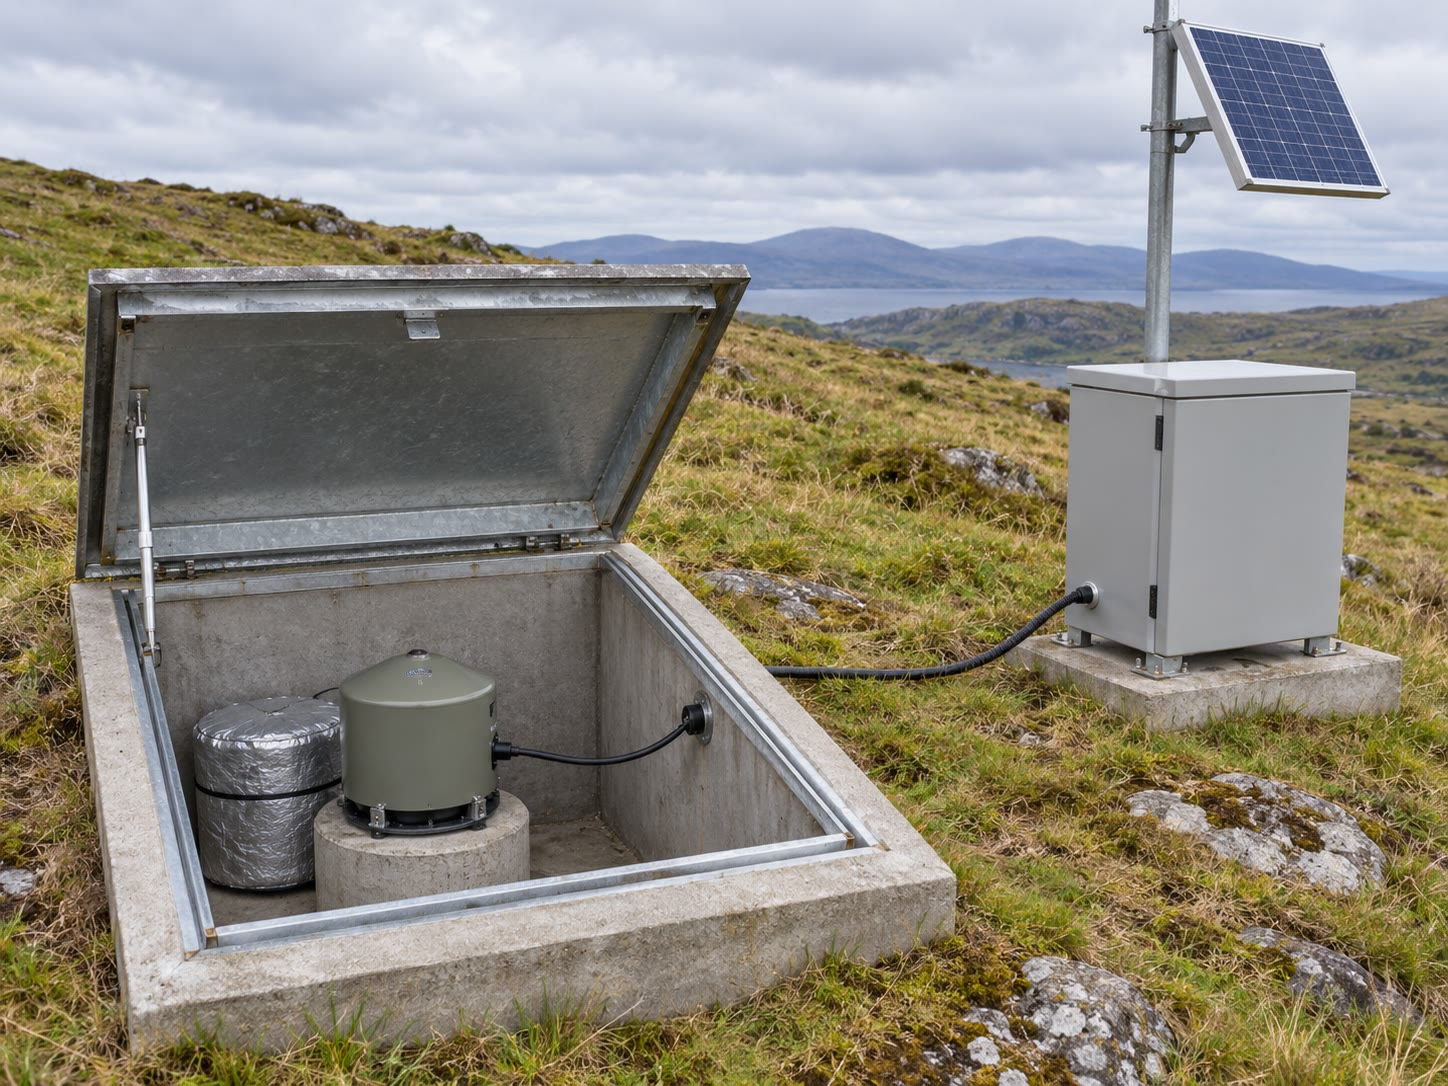
\includegraphics[width=\linewidth]{images/book5/ai/b3-seismic-vault.jpg}

{\scriptsize Sismómetro de banda ancha sobre su pilar en una cámara de estación
Ilustración generada por IA.}
\end{minipage}
\end{inthefield}

\section{Ejercicios}

\begin{exercise}[$\star$]\label{exo:b3:seismology-imaging:1}
Un rayo P sale de la superficie ($R = \qty{6371}{km}$, $v_0 = \qty{5.80}{km.s^{-1}}$)
con el \omterm{def:b3:seismology-imaging:ray-parameter}{parámetro del rayo} $p = \qty{500}{s.rad^{-1}}$. (a) Calcúlese su ángulo de
salida. (b) PREM da velocidades P de \qty{11.066}{km.s^{-1}} a \qty{771}{km} de profundidad
y \qty{11.245}{km.s^{-1}} a \qty{871}{km}. Calcúlese $r/v$ a ambas profundidades y
hállese la profundidad del punto de retorno del rayo por interpolación lineal.
% ledger: ak135:crust, data:prem
\end{exercise}

\begin{exercise}[$\star$]\label{exo:b3:seismology-imaging:2}
Los tiempos P calculados con PREM en este capítulo son \qty{369.6}{s} a \ang{30}
y \qty{455.5}{s} a \ang{40}. (a) Estímese la pendiente de la curva de tiempos de recorrido
entre ellos, en \unit{s} por grado y en \unit{s.rad^{-1}}. (b) Dedúzcase
la velocidad aparente del frente de onda a lo largo de la superficie, en
\unit{km.s^{-1}}. (c) ¿Cuál es la velocidad P en el punto de retorno del rayo
que llega a \ang{35}, si su punto de retorno está en el radio \qty{5450}{km}?
\end{exercise}

\begin{exercise}[$\star$]\label{exo:b3:seismology-imaging:3}
En el modelo de \omterm{def:b3:seismology-imaging:surface-waves}{onda de Love} de este capítulo la capa tiene $\beta_1 =
\qty{3.5}{km.s^{-1}}$, $\rho_1 = \qty{2700}{kg.m^{-3}}$ y el semiespacio
$\beta_2 = \qty{4.5}{km.s^{-1}}$, $\rho_2 = \qty{3300}{kg.m^{-3}}$.
(a) Calcúlense los dos módulos de cizalla. (b) A \qty{20}{s} la velocidad de fase es
\qty{3.79}{km.s^{-1}}: calcúlese la longitud de onda y compárese con el espesor de la capa,
\qty{35}{km}. (c) Con velocidades de grupo de \qty{3.384}{km.s^{-1}} a
\qty{20}{s} y \qty{4.333}{km.s^{-1}} a \qty{100}{s}, ¿en cuántos minutos llegan
las ondas de 20 s después de las de 100 s en una estación situada a \qty{4000}{km}?
\end{exercise}

\begin{exercise}[$\star$]\label{exo:b3:seismology-imaging:4}
Los periodos observados de ${}_0S_2$ y ${}_0T_2$ son \qty{53.89}{min} y
\qty{44.01}{min}. (a) Calcúlense sus frecuencias en \unit{mHz}. (b) ¿Cuántas
oscilaciones de cada uno completa la Tierra en un día? (c) Dos picos espectrales
pueden separarse solo si el registro dura al menos el inverso de su
diferencia de frecuencias. ¿Cuánto debe durar un registro para separar estos dos modos?
% ledger: seis5:modes-S, seis5:modes-T
\end{exercise}

\begin{exercise}[$\star\star$]\label{exo:b3:seismology-imaging:5}
En una esfera de radio $R$ y velocidad uniforme $v$ los rayos son cuerdas rectas.
(a) Demuéstrese que el rayo que llega a $\Delta$ tiene el tiempo de recorrido
$T = 2R\sin(\Delta/2)/v$. (b) Con $R = \qty{6371}{km}$ y
$v = \qty{10.0}{km.s^{-1}}$, calcúlese $T$ a \ang{30} y \ang{90}, y compárese
con los tiempos de PREM, \qty{369.6}{s} y \qty{779.7}{s}. (c) Explíquese por qué la
esfera uniforme es demasiado rápida a \ang{30} y demasiado lenta a \ang{90}.
\end{exercise}

\begin{exercise}[$\star\star$]\label{exo:b3:seismology-imaging:6}
En un sólido de Poisson ($\lambda = \mu$, luego $\alpha^2 = 3\beta^2$) la \omterm{def:b3:seismology-imaging:surface-waves}{onda de Rayleigh}
de velocidad $c$ satisface, con $\xi = c^2/\beta^2$,
$(2 - \xi)^2 = 4\sqrt{1 - \xi/3}\,\sqrt{1 - \xi}$. (a) Elévese al cuadrado y demuéstrese
que las raíces satisfacen $(\xi - 4)(3\xi^2 - 12\xi + 8) = 0$. (b) Demuéstrese que la
única raíz con $0 < \xi < 1$ es $\xi = 2 - 2/\sqrt3$, y calcúlese $c/\beta$.
(c) En la corteza superior de ak135, $\beta = \qty{3.46}{km.s^{-1}}$: calcúlese la
velocidad de Rayleigh y el retraso de la \omterm{def:b3:seismology-imaging:surface-waves}{onda de Rayleigh} respecto de la onda S a
\qty{1000}{km}.
% ledger: ak135:crust
\end{exercise}

\begin{exercise}[$\star\star$]\label{exo:b3:seismology-imaging:7}
Las llegadas de onda de cabeza en cuatro estaciones de una línea de refracción, a 50, 100, 150 y
\qty{200}{km} del disparo, son 9.0, 15.3, 21.5 y \qty{27.9}{s}, con
errores de 0.1, 0.1, 0.2 y \qty{0.2}{s}. Ajústese $T = a + bx$ por mínimos cuadrados
ponderados: escríbanse $\mathsf G$ y $\mathsf C_d$, fórmense las ecuaciones normales y
dense $a$, $b$, sus errores estándar, la velocidad $1/b$ con su error y el
mínimo $\chi^2$. ¿Es aceptable el ajuste?
\end{exercise}

\begin{exercise}[$\star\star$]\label{exo:b3:seismology-imaging:8}
Un rayo atraviesa dos celdas, de longitudes \qty{30}{km} y \qty{40}{km}, y tiene
un residuo de \qty{0.50}{s}. (a) ¿Por qué es singular $\mathsf N = \mathsf G^{\mathsf T}
\mathsf G$? (b) Entre los modelos que ajustan el residuo exactamente, el de
menor norma es $\mathbf m = \mathsf G^{\mathsf T}(\mathsf G\mathsf
G^{\mathsf T})^{-1}\mathbf d$: calcúlese. (c) Calcúlese la matriz
$\mathsf R = \mathsf G^{\mathsf T}(\mathsf G\mathsf G^{\mathsf T})^{-1}\mathsf G$
y su traza. (d) Si la anomalía verdadera es \qty{0.01}{s.km^{-1}} solo en la primera
celda, ¿qué se recupera?
\end{exercise}

\begin{exercise}[$\star\star$]\label{exo:b3:seismology-imaging:9}
Una región de losa del manto es un \qty{3}{\percent} más rápida que su entorno,
donde $v = \qty{9.0}{km.s^{-1}}$. (a) Calcúlese el residuo de un rayo que atraviesa
\qty{200}{km} de ella en vertical, mediante la \cref{prop:b3:seismology-imaging:linear},
y de forma exacta. (b) Lo mismo para un rayo que atraviesa un espesor de \qty{100}{km} de ella con un ángulo de
\ang{40} respecto a la normal a la losa. (c) ¿Cuál es el error relativo de la
linealización?
\end{exercise}

\begin{exercise}[$\star\star\star$]\label{exo:b3:seismology-imaging:10}
En el \cref{thm:b3:seismology-imaging:love}, un sobretono de orden $n$ existe solo
para periodos suficientemente cortos. (a) Demuéstrese que en su frecuencia de corte la velocidad de fase es
$\beta_2$ y $kHq_1 = n\pi$. (b) Dedúzcase la frecuencia angular de corte
$\omega_n = n\pi\beta_1\beta_2/\bigl(H\sqrt{\beta_2^2 - \beta_1^2}\bigr)$.
(c) Calcúlese el periodo de corte del primer sobretono para el modelo del capítulo
($H = \qty{35}{km}$, $\beta_1 = 3.5$, $\beta_2 = \qty{4.5}{km.s^{-1}}$).
(d) Demuéstrese que el modo fundamental no tiene frecuencia de corte y que su velocidad de fase
tiende a $\beta_1$ para periodos cortos.
\end{exercise}

\begin{exercise}[$\star\star\star$]\label{exo:b3:seismology-imaging:11}
Tómese el rayo del ejercicio 8, con error de datos unitario. (a) Demuéstrese que, para cualquier
$\varepsilon > 0$, $(\mathsf G^{\mathsf T}\mathsf G + \varepsilon^2\mathsf
I)^{-1}\mathsf G^{\mathsf T} = \mathsf G^{\mathsf T}(\mathsf G\mathsf
G^{\mathsf T} + \varepsilon^2\mathsf I)^{-1}$. (b) Dedúzcase la
matriz de resolución amortiguada $\mathsf R_\varepsilon = \mathsf G^{\mathsf T}\mathsf G/(\|\mathbf g\|^2 +
\varepsilon^2)$, donde $\mathbf g = (30, 40)$, y su traza. (c) Calcúlese la
traza y el residuo de datos para $\varepsilon^2 = 0$, 2500 y \num{10000}
(en \unit{km^2}). Descríbase el compromiso.
\end{exercise}

\begin{exercise}[$\star\star\star$]\label{exo:b3:seismology-imaging:12}
En la esfera uniforme del ejercicio 5: (a) demuéstrese mediante
el \cref{thm:b3:seismology-imaging:benndorf} que $p(\Delta) = (R/v)\cos(\Delta/2)$,
y compruébese con la definición de $p$ (el ángulo de salida de una cuerda).
(b) Demuéstrese que el rayo que llega a $\Delta_1$ tiene su punto de retorno en $r_1 = R\cos(\Delta_1/2)$.
(c) Admitiendo que $\int_0^{\Delta_1}\operatorname{arccosh}\bigl(\cos(\Delta/2)
/\cos(\Delta_1/2)\bigr)\,\mathrm d\Delta = \pi\ln\bigl(1/\cos(\Delta_1/2)\bigr)$,
demuéstrese que la fórmula de Herglotz--Wiechert devuelve $r_1$ y la velocidad $v$.
\end{exercise}

\section{Problema: la losa bajo la estación K}

\begin{problem}[{Problema de fin de semana --- rayos, ondas de Love y una pequeña tomografía
bajo una estación ficticia}]
\label{pb:b3:seismology-imaging:1}
% values: calc/ch01.py (invented station and models; Love-wave model as in the chapter)
La estación K se sitúa sobre un continente, encima de una zona de subducción. Este problema emplea sus
registros de tres maneras: rayos en su corteza, la dispersión de las \omterm{def:b3:seismology-imaging:surface-waves}{ondas de Love} a través de ella,
y una pequeña tomografía del manto subyacente.

\medskip
\noindent\textbf{Parte I --- Rayos en un gradiente.} A distancias lo bastante cortas para despreciar la curvatura terrestre,
la velocidad de las ondas P bajo K aumenta linealmente con la profundidad,
$v(z) = v_0 + gz$, con $v_0 = \qty{5.0}{km.s^{-1}}$ y
$g = \qty{0.05}{s^{-1}}$ ($z$ en km).
\begin{enumerate}
  \item En capas planas, la ley de Snell mantiene constante $p = \sin i/v$. Un rayo sale
        K con $\sin i_0 = 0.8$: calcúlense $i_0$ y $p$.
  \item ¿A qué profundidad tiene su punto de retorno, y cuál es allí la velocidad?
  \item Demuéstrese que $\mathrm di/\mathrm ds = pg$ a lo largo del rayo, de modo que es un
        arco de circunferencia; dése su radio y la profundidad de su centro.
  \item Calcúlese la distancia horizontal $X$ a la que el rayo regresa a la
        superficie.
  \item Demuéstrese que $\mathrm dT = \mathrm di/(g\sin i)$ y calcúlese el tiempo de
        recorrido $T$ de forma exacta.
  \item Calcúlense $X$ y $T$ para $p = \qty{0.15}{s.km^{-1}}$, y compruébese que
        $\Delta T/\Delta X$ entre los dos rayos está comprendido entre los dos valores
        de $p$.
\end{enumerate}

\noindent\textbf{Parte II --- Ondas de Love y la corteza.} La corteza bajo K es una capa
de velocidad S $\beta_1 = \qty{3.5}{km.s^{-1}}$ y densidad
$\rho_1 = \qty{2.7}{g.cm^{-3}}$ sobre un manto con $\beta_2 =
\qty{4.5}{km.s^{-1}}$, $\rho_2 = \qty{3.3}{g.cm^{-3}}$; su espesor $H$ es
desconocido. Entre K y una estación vecina la velocidad de fase de las \omterm{def:b3:seismology-imaging:surface-waves}{ondas de Love}
se mide: \qty{3.99}{km.s^{-1}} a \qty{25}{s} y \qty{4.25}{km.s^{-1}} a
\qty{40}{s}.
\begin{enumerate}[resume]
  \item Calcúlense $\mu_1$ y $\mu_2$ en \unit{GPa}.
  \item A \qty{25}{s}, calcúlense $k$, $q_1$ y $q_2$.
  \item Resuélvase la ecuación de dispersión del modo fundamental para $H$.
  \item Repítase lo mismo a \qty{40}{s}. ¿Son consistentes los dos resultados?
  \item Estímese la velocidad de grupo entre los dos periodos como
        $\Delta\omega/\Delta k$, y compárese con las velocidades de fase.
  \item Calcúlese la longitud de onda a cada periodo y explíquese por qué los dos periodos
        sondean la corteza y el manto superior en
        distinta proporción.
\end{enumerate}

\noindent\textbf{Parte III --- Una tomografía en cuatro celdas.} Bajo K, un bloque de
manto de \qty{200}{km} por \qty{200}{km} en una sección vertical se divide en cuatro
celdas cuadradas de \qty{100}{km}: 1 (superior izquierda), 2 (superior derecha), 3 (inferior izquierda)
y 4 (inferior derecha); la fosa y el océano quedan a la izquierda. La velocidad de referencia es $v_0 = \qty{8.0}{km.s^{-1}}$. En un
experimento idealizado, seis rayos rectos la atraviesan: A a lo largo de la fila superior (celdas 1
y 2), B a lo largo de la fila inferior (3 y 4), C por la columna izquierda (1 y 3), D
por la columna derecha (2 y 4), E a lo largo de la diagonal por 1 y 4, F a lo largo de
la diagonal por 2 y 3. Sus residuos son:
\begin{center}
\small
\begin{tabular}{lcccccc}
\hline
rayo & A & B & C & D & E & F \\
$\delta t$ (\unit{s}) & $0.16$ & $-0.48$ & $-0.36$ & $0.11$ & $-0.15$ & $-0.27$ \\
error $\sigma$ (\unit{s}) & 0.05 & 0.05 & 0.05 & 0.05 & 0.10 & 0.10 \\
\hline
\end{tabular}
\end{center}
El modelo $\mathbf m$ se toma como las perturbaciones de lentitud de las celdas en
\unit{ms.km^{-1}} ($\qty{1}{ms.km^{-1}} = \qty{e-3}{s.km^{-1}}$), de modo que las
entradas de $\mathsf G$ son las longitudes de los rayos en \unit{km} divididas entre 1000.
\begin{enumerate}[resume]
  \item Escríbase $\mathsf G$, una matriz $6\times4$.
  \item Demuéstrese que $\mathsf N = \mathsf G^{\mathsf T}\mathsf C_d^{-1}\mathsf G$
        tiene las filas $(10, 4, 4, 2)$, $(4, 10, 2, 4)$, $(4, 2, 10, 4)$,
        $(2, 4, 4, 10)$.
  \item Calcúlese $\mathbf b = \mathsf G^{\mathsf T}\mathsf C_d^{-1}\mathbf d$.
  \item Compruébese que $(1,1,1,1)$, $(1,-1,-1,1)$, $(1,1,-1,-1)$ y $(1,-1,1,-1)$
        son autovectores de $\mathsf N$, con autovalores 20, 4, 8 y 8, y
        dedúzcase que $\mathsf N^{-1}$ tiene las filas $(11, -4, -4, 1)/80$,
        $(-4, 11, 1, -4)/80$, $(-4, 1, 11, -4)/80$ y $(1, -4, -4, 11)/80$.
  \item Calcúlese la \omterm{thm:b3:seismology-imaging:wls}{estimación por mínimos cuadrados ponderados} $\hat{\mathbf m}$.
  \item Conviértase en anomalías relativas de velocidad $\delta v/v_0$ en por ciento.
  \item Dése el error estándar de cada celda en \unit{ms.km^{-1}} y en por
        ciento, y la correlación entre las celdas 1 y 2, y entre las celdas 1
        y 4. Explíquense sus signos.
  \item Calcúlense los residuos de los seis rayos tras el ajuste y el mínimo
        $\chi^2$. ¿Es compatible con los errores indicados?
\end{enumerate}

\noindent\textbf{Parte IV --- Amortiguamiento, resolución y la losa.}
\begin{enumerate}[resume]
  \item Para $\varepsilon^2 = 4$ (en las unidades de $\mathsf N$), dense los
        autovalores de $\mathsf R = (\mathsf N + 4\mathsf I)^{-1}\mathsf N$ y
        demuéstrese que $\mathsf R$ tiene la diagonal $2/3$, las entradas $1/12$
        entre celdas que comparten un rayo de fila o de columna, y $0$ entre las celdas 1
        y 4, y entre las celdas 2 y 3.
  \item Calcúlese la estimación amortiguada de la celda 3 y su anomalía de velocidad. ¿Por qué es
        menor que la estimación sin amortiguar?
  \item El modelo amortiguado tiene $\chi^2 = 15.8$ y norma \qty{2.91}{ms.km^{-1}};
        el no amortiguado, $\chi^2 = 0.50$ y \qty{4.24}{ms.km^{-1}}. ¿Cuál se
        conservaría, y por qué este problema no necesita amortiguamiento?
  \item Léase la fila 3 de $\mathsf R$ amortiguada: ¿con qué celdas
        se mezcla la estimación de la celda 3?
  \item ¿Cuál celda es rápida y cuál lenta? Interprétese la celda rápida, debajo y
        del lado del océano de K, en términos de la zona de subducción.
  \item Dése la anomalía de velocidad P de la celda de la losa en por ciento, con su
        error estándar.
\end{enumerate}
\end{problem}
